\documentclass[letterpaper, 12pt]{article}

\usepackage{graphicx}
\usepackage{fancyhdr}
\usepackage[T1]{fontenc}
\usepackage{lmodern}
\usepackage[francais]{babel}
\usepackage{lipsum}
\usepackage{vmargin}
\usepackage{lastpage}
\usepackage{enumerate}
\usepackage{pdfpages}
\usepackage[nogin]{Sweave}
\usepackage{lscape}
\usepackage{color}
\usepackage{listings}
\usepackage{verbatim}
\usepackage{wrapfig}
\usepackage{hyperref}
\usepackage{parskip}
\usepackage{amssymb, amsmath}


\begin{document}

\begin{titlepage}
\vspace*{3cm}
\begin{center}

\huge{\bf Type of relation for probabilities}\\
\huge{\bf Package `bmisc'}\\
\vspace*{2cm}
\large{By Beno�t Bruneau}
\end{center}
\vspace*{4cm}

%\hangindent=1cm
%\begin{flushleft}
\begin{description}
\item[Package:] `bmisc'
\item[Version:] 0.2-12
\item[Depends:] car, lattice, zoo, robustbase, and methods
\item[Author \& Maintainer:] Benoit Bruneau (\href{mailto:benoit.bruneau1@gmail.com}{benoit.bruneau1@gmail.com})
\item[Description:] These functions can be used to estimate probabilities \verb=[0,1]= by specifying the inflection points of a relation. Described relations are of type `full',`ramp' and `logistic'.
\item[License:] LGPL $\geqslant$ 3.0
\end{description}


\vspace*{\fill;}


\end{titlepage}

\tableofcontents
\newpage

\section{Type full and plat.full probabilities}
%\noindent These relations have "all-or-nothing" types of probabilities. 

%\begin{description}
%\item[\verb=full.sel=] \verb=(infl1,x)=
%\item{\verb=plat.full.sel=]\verb=(infl1,infl2,x)=
%\end{description}

\begin{Schunk}
\begin{Sinput}
> data = 0:3000
> res1 = full.sel(infl1 = 1500, x = data)
> plot(res1 ~ data, type = "l", lwd = 2, col = "blue", main = "Type 'full'")
\end{Sinput}
\end{Schunk}

\begin{center}
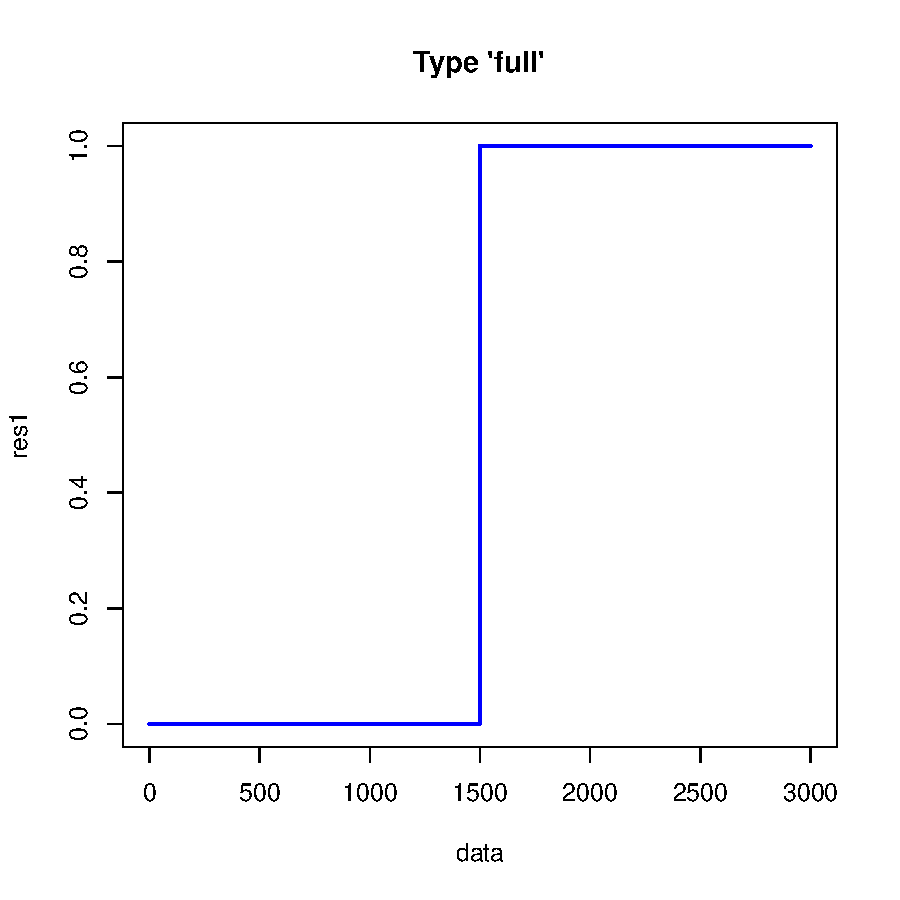
\includegraphics{relation_sel-002}
\end{center}

\begin{Schunk}
\begin{Sinput}
> e = rnorm(1000)
> mysummary <- function(x, npar = TRUE, print = TRUE) {
     if (!npar) {
         center <- mean(x)
         spread <- sd(x)
     }
     else {
         center <- median(x)
         spread <- mad(x)
     }
     if (print & !npar) {
         cat("Mean=", center, "\n", "SD=", spread, "\n")
     }
     else if (print & npar) {
         cat("Median=", center, "\n", "MAD=", spread, "\n")
     }
     result <- list(center = center, spread = spread)
     return(result)
 }
\end{Sinput}
\end{Schunk}

\noindent Exemple d'utilisation de cette fonction:  
\begin{Schunk}
\begin{Sinput}
> set.seed(1234)
> x <- rpois(500, 4)
> y <- mysummary(x)
\end{Sinput}
\begin{Soutput}
Median= 4 
 MAD= 1.4826 
\end{Soutput}
\end{Schunk}




\begin{center}
\noindent \large{ \bf Le pr�sent document est appel� � �voluer.}
\end{center}

       
\end{document}
